\chapter{Appendix}
\textbf{English stop words} \\
\input{appendix/english_word_stops.txt}
\begin{figure}[H]
\centering
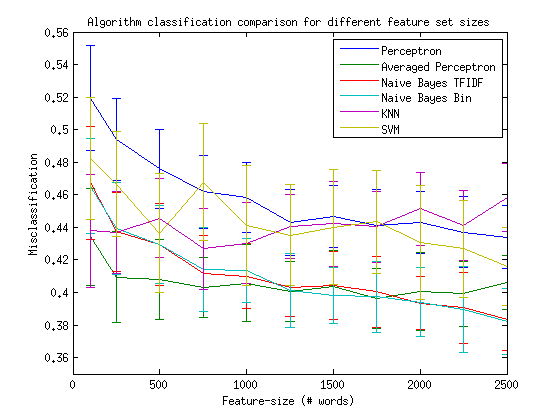
\includegraphics[scale = 0.5]{../Plottar/feature-size100-2500bigram.png}
\caption{In-domain classification using varying Bigram feature set sizes with 2$\sigma$ height error bars and comparing all algorithms.}
\label{fig:trainingsize}
\end{figure} 

\begin{figure}[H]
\centering
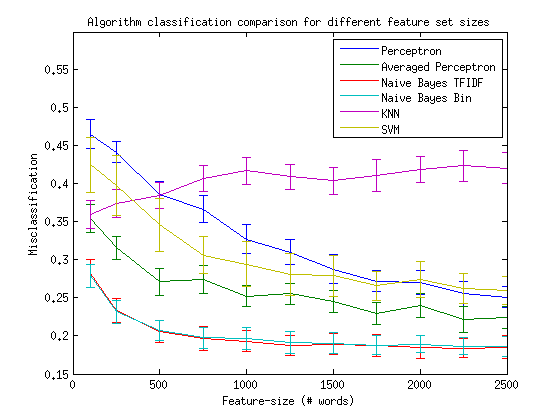
\includegraphics[scale = 0.5]{../Plottar/feature-size100-2500all.png}
\caption{In-domain classification using varying Bigram feature set sizes with 2$\sigma$ height error bars and comparing all algorithms.}
\label{fig:trainingsize}
\end{figure} 

\begin{figure}[H]
\centering
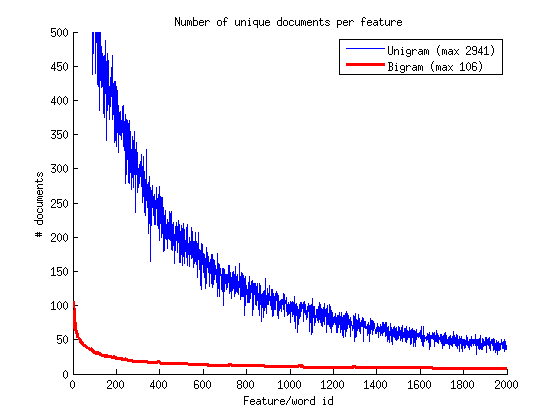
\includegraphics[scale = 0.5]{../Plottar/documents_per_feature.png}
\caption{Documents per feature. Bigram and Unigram.}
\label{fig:trainingsize}
\end{figure} 

\begin{figure}[H]
\centering
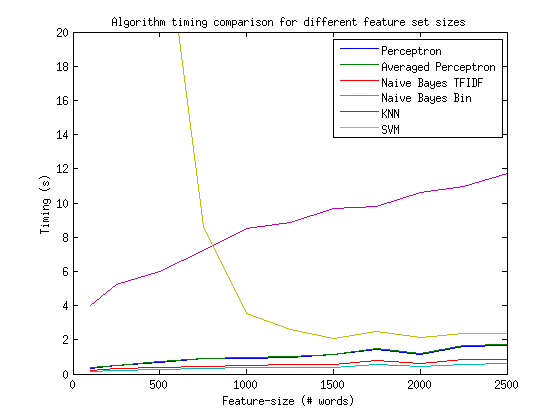
\includegraphics[scale = 0.5]{../Plottar/feature_size_TIMING.png}
\caption{Timing of different algorithms with different feature sizes}
\label{fig:trainingsize}
\end{figure} 

\begin{figure}[H]
\centering
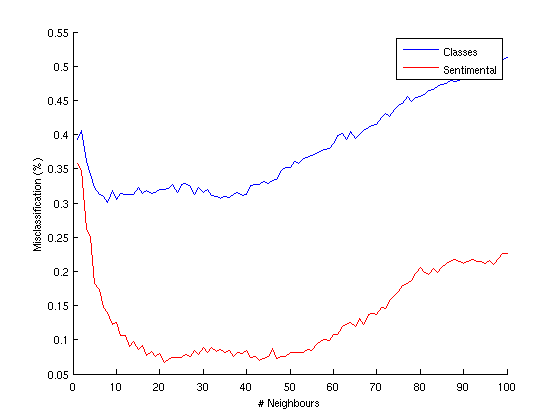
\includegraphics[scale = 0.5]{../Plottar/knn_2000words_testdata100_unigram.png}
\caption{Different K-values when running KNN on Classes and Sentimental-label}
\label{fig:trainingsize}
\end{figure} 


\begin{figure}[H]
\centering
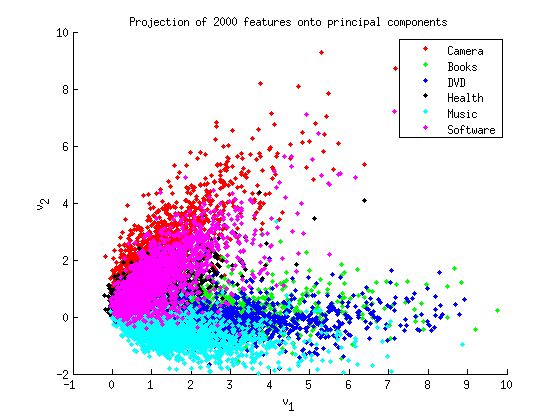
\includegraphics[scale = 0.5]{../Plottar/pca_all.png}
\caption{PCA on all categories}
\label{fig:trainingsize}
\end{figure} 

\begin{figure}[H]
\centering
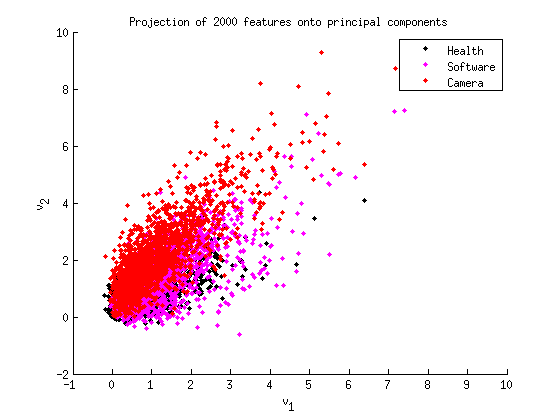
\includegraphics[scale = 0.5]{../Plottar/pca_largecorr.png}
\caption{PCA on health, software and camera. Represent a large correlation}
\label{fig:trainingsize}
\end{figure} 

\begin{figure}[H]
\centering
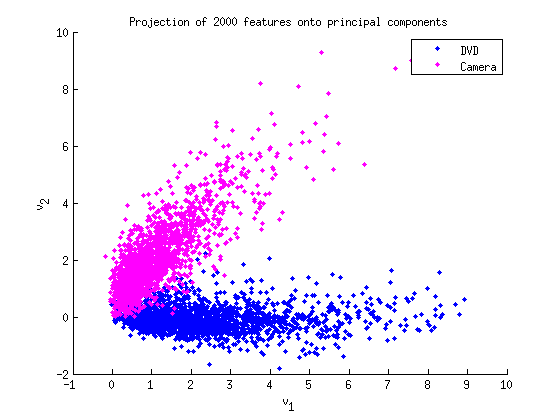
\includegraphics[scale = 0.5]{../Plottar/pca_nocorr.png}
\caption{PCA on DVD and camera with no correlation}
\label{fig:trainingsize}
\end{figure} 

\begin{figure}[H]
\centering
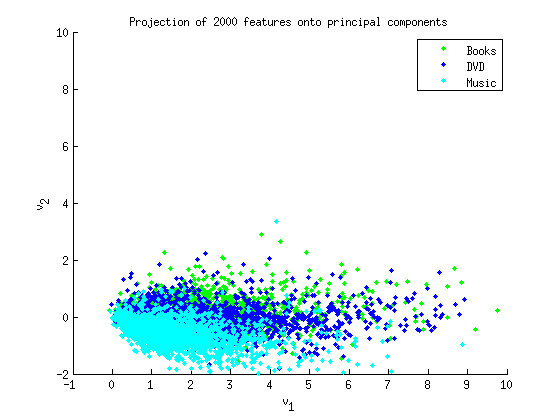
\includegraphics[scale = 0.5]{../Plottar/pca_somecorr.png}
\caption{PCA on Books, DVD and Music with some correlation}
\label{fig:trainingsize}
\end{figure} 

\begin{figure}[H]
\centering
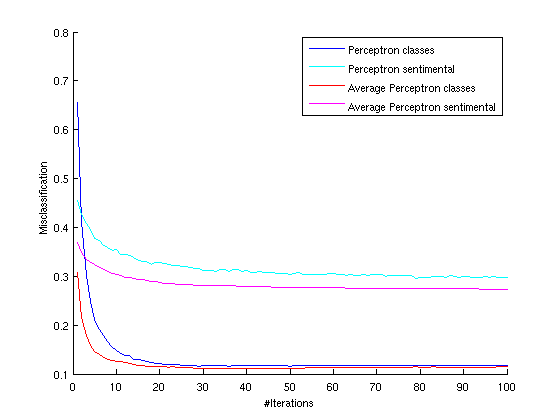
\includegraphics[scale = 0.5]{../Plottar/perceptron_2000words_unigram_10foldcv_classes-high_sentimental-low.png}
\caption{Different max iteration Perceptron}
\label{fig:trainingsize}
\end{figure} 

\begin{figure}[H]
\centering
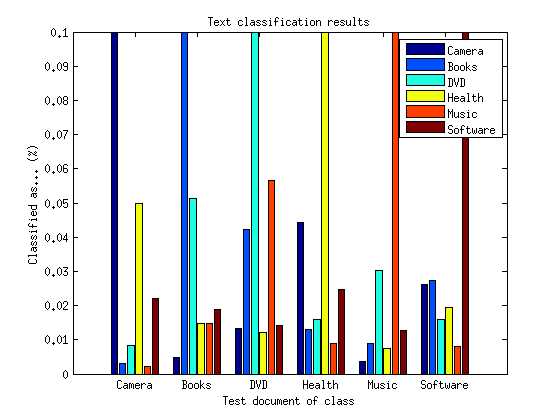
\includegraphics[scale = 0.3]{../Plottar/text_categorization.png}
\caption{Text categorization task}
\label{fig:trainingsize}
\end{figure} 

\begin{figure}[H]
\centering
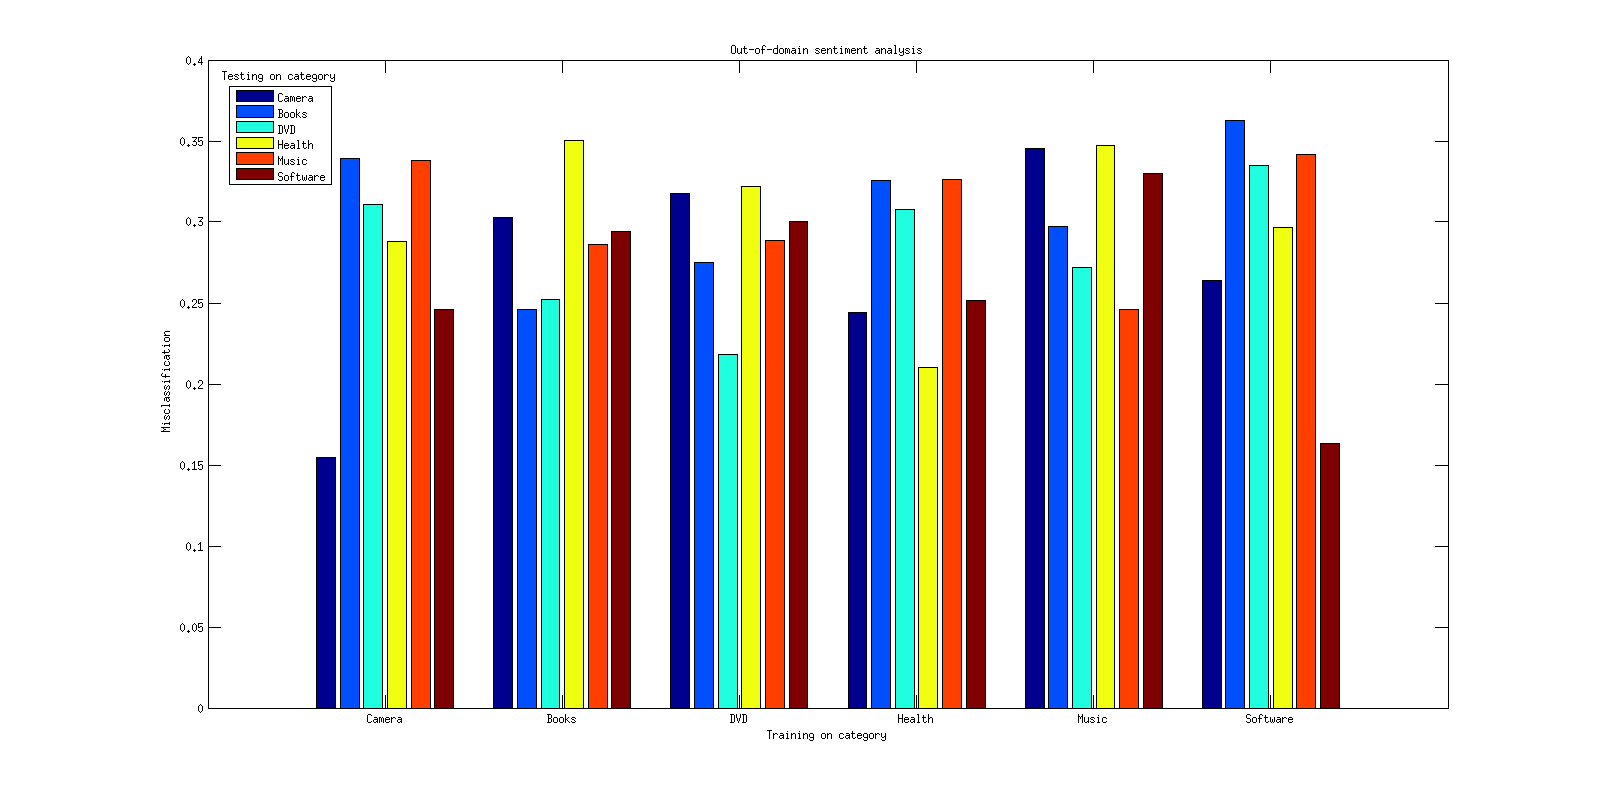
\includegraphics[scale = 0.3]{../Plottar/outofdomain.png}
\caption{Out of domain classification task}
\label{fig:trainingsize}
\end{figure} 



\begin{figure}[H]
\centering
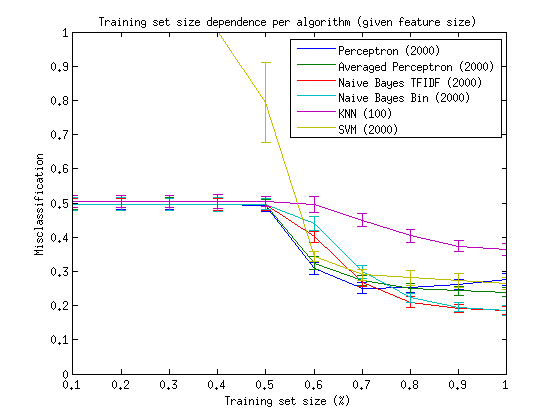
\includegraphics[scale = 0.8]{../Plottar/training_size_k_2000allknn_100.png}
\caption{Training set size dependence per algorithm}
\label{fig:trainingsize}
\end{figure} 
\newpage
\textbf{Individual Page - Oscar Carlsson} \\\\
I've been sort of trying to act project manager, involving dividing equally amount of work on each group member and steering the project in the right direction. I've taught some basics in git in the beginning of the project and managed the repository with branches and such to make the the work easier for the others. All of us were new to Git so this has required some reading and supporting. \\\\
We wrote alot in teams and everyone has almost certainly edited every file some time during the project, but i will try to state which areas i've been most involved in. \\\\
We set up some scripts to process the documents into Matlab-friendly vectors. I contributed with a Snowball-stemmer, handling of arguments and pair-programmed TF-IDF etc. I were also involved in creating a nice way of generating feature vectors in .mat-format (such that all algorithms only needed to load the work space). Dealed with most areas of the datamanipulation.\\\\
All of us had prior knowledge of Machine Learning and we were able to re-use a lot of Matlab code. The original perceptron algorithm was at first written by me, but later on changed. I helped writing code to perform the classification tasks: In domain sentimental, Out of domain sentimental and Text categorization. Also spent some time to get nice plots of the data we received from the tests.\\\\
I started a lot of big and heavy tests on some of the computers at school. Started, collected data and made re-runs if there were any errors. E.g Training size-plot and Feature size-plot, both bigram and unigram.\\\\
In te final report i had the resposiblity for the parts related to Support Vector Machines, the paragraph about cross validation and wrote about our conclusions. But i, like the others, have been editing and writing in most of the chapters.\\\\
